\subsubsection{Cache Structure}

Each entry (cache line) in the cache includes:
\begin{itemize}
    \item (\textbf{V}) \textbf{Valid bit} to indicate if this position contains valid data or not. At the bootstrap, all the entries in the cache are marked as \texttt{INVALID}.

    \item (\textbf{TAG}) \textbf{Cache Tag(s)} contains the value that univocally identifies the memory address corresponding to the stored data.

    \item (\textbf{DATA}) \textbf{Cache Data} contains a copy of data (block or cache line).
\end{itemize}
\begin{figure}[!htp]
    \centering
    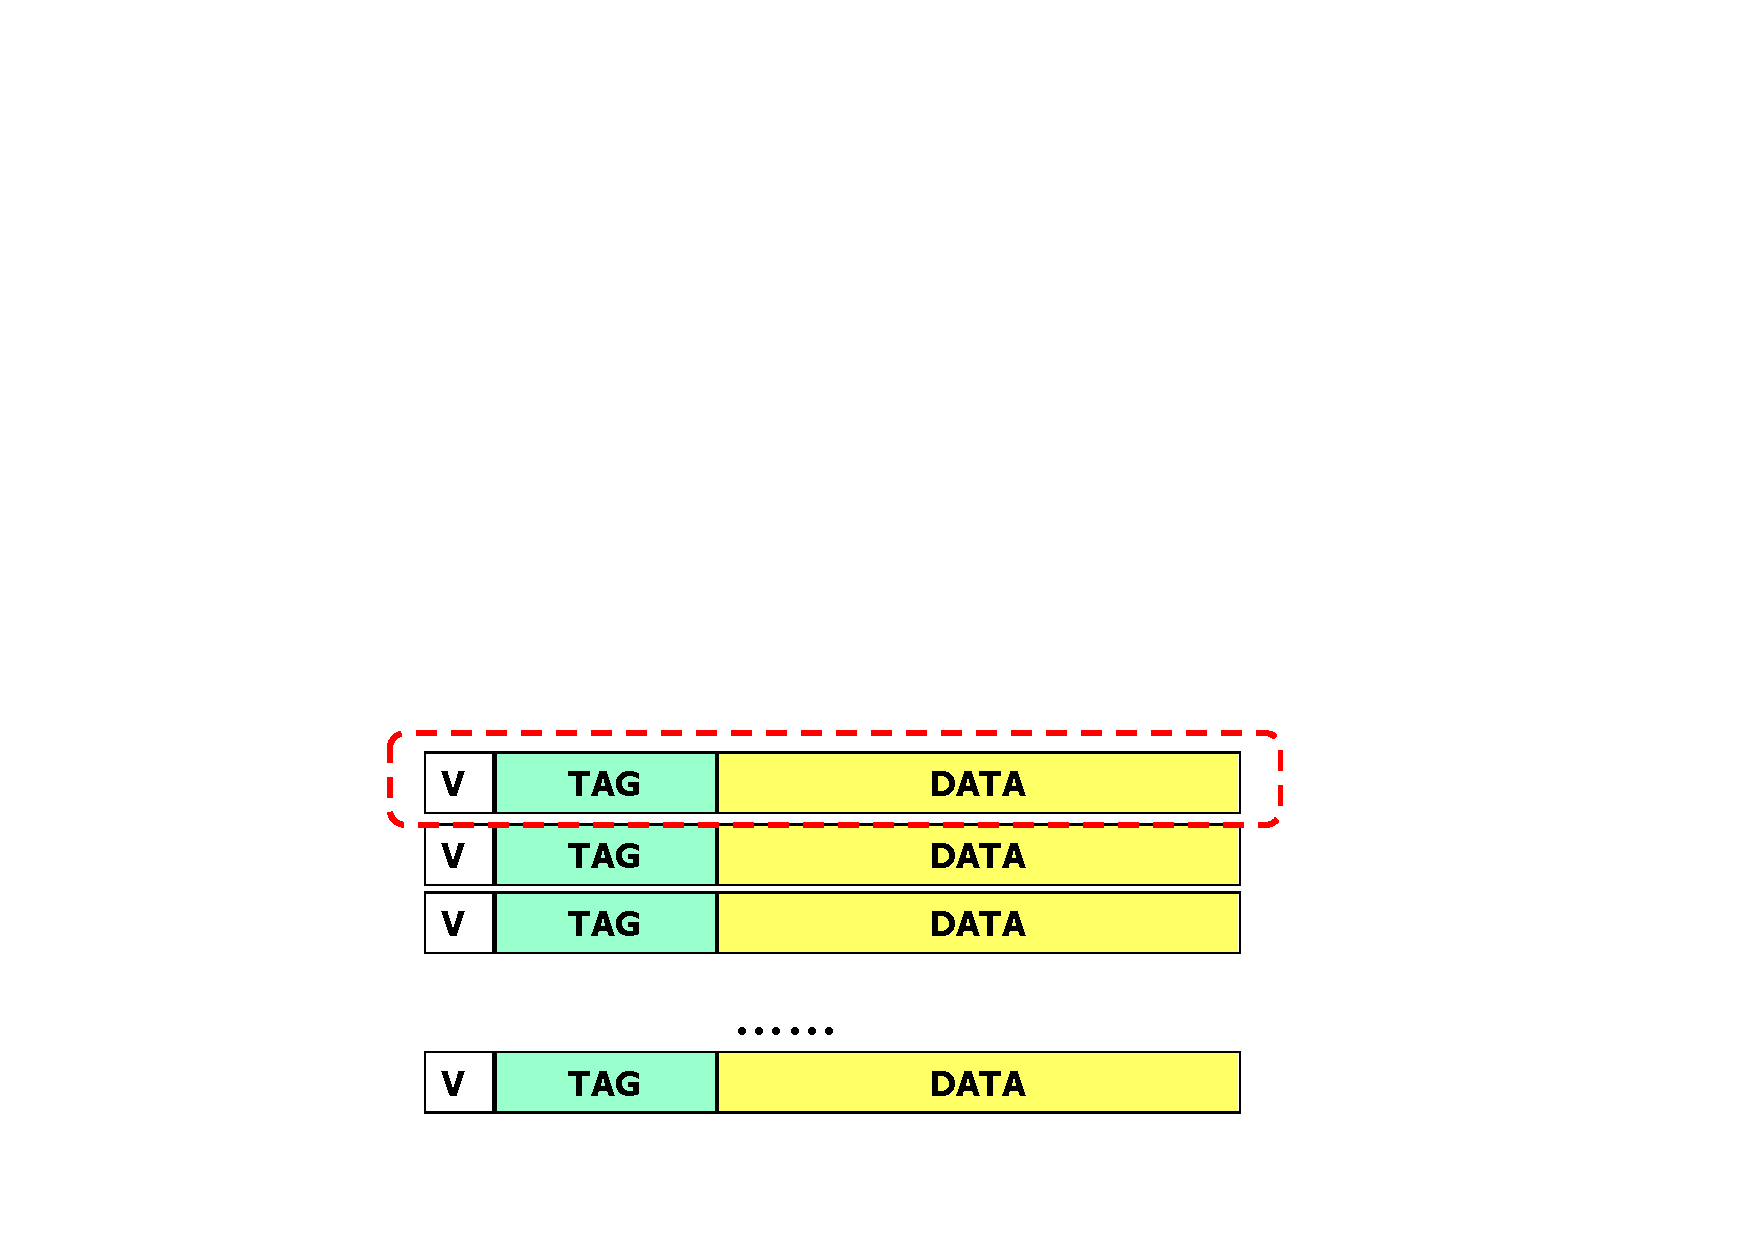
\includegraphics[width=.7\textwidth]{img/cache-structure-1.pdf}
\end{figure}

\noindent
After a general presentation of the cache structure, we answer four questions about the memory hierarchy to understand different topics: 
\begin{itemize}
    \item \textbf{Block placement} (page~\hyperlink{Block placement}{\hypergetpageref{Block placement}}). \emph{Where can a block be placed in the upper level?}
    \begin{itemize}
        \item Direct Mapped Cache (page~\hyperlink{Direct Mapped Cache}{\hypergetpageref{Direct Mapped Cache}})

        \item Fully Associative Cache (page~\hyperlink{Fully Associative Cache}{\hypergetpageref{Fully Associative Cache}})
        
        \item \emph{n}-way Set Associative Cache (page~\hyperlink{n-way Set Associative Cache}{\hypergetpageref{n-way Set Associative Cache}})
    \end{itemize}
    
    \item \textbf{Block identification} (page~\hyperlink{Block identification}{\hypergetpageref{Block identification}}). \emph{How is a block found if it is in the upper level?}
    
    \item \textbf{Block replacement} (page~\hyperlink{Block replacement}{\hypergetpageref{Block replacement}}). \emph{Which block should be replaced on a miss?}
    
    \item \textbf{Write strategy} (page~\hyperlink{Write strategy}{\hypergetpageref{Write strategy}}). \emph{What happens on a write?}
\end{itemize}

\newpage

\begin{center}
    \large
    \label{Block placement}
    \hypertarget{Block placement}{\textcolor{Red2}{\textbf{Block placement}}}
\end{center}

\noindent
The main question is: \emph{where can a block be placed in the upper level?} In other words, the problem is: given the address of the block in the main memory, \textbf{where can the block be placed in the cache}?

\highspace
So, we need to find the \textbf{correspondence between the memory address and the cache address of the block}. This correspondence \textbf{depends on the cache structure} and can be of three types:
\begin{itemize}
    \item \textbf{Direct Mapped Cache}
    \item \textbf{Fully Associative Cache}
    \item \textbf{\emph{n}-way Set-Associative Cache}
\end{itemize}

\label{Direct Mapped Cache}
\hypertarget{Direct Mapped Cache}{\subsubsection*{\textcolor{Red2}{Direct Mapped Cache}}}

With the \definition{Direct Mapped Cache} structure, \textbf{each memory location corresponds to one cache location and only one cache location}. The following formula gives the \textbf{cache address of the block}:
\begin{equation}\label{eq: direct mapped cache}
    \left(\texttt{Block Address}\right)_{\texttt{cache}} = \left(\texttt{Block Address}\right)_{\texttt{mem}} \texttt{mod} \left(\texttt{\# Cache Blocks}\right)
\end{equation}
The \emph{block address} of the \emph{cache} corresponds to the modulo operation between the \emph{block address} of the \emph{memory} and the \emph{number} (\#) \emph{of cache blocks}. The \href{https://en.wikipedia.org/wiki/Modulo}{modulo operation} returns a division's remainder or signed remainder after dividing one number by another.

\begin{figure}[!htp]
    \centering
    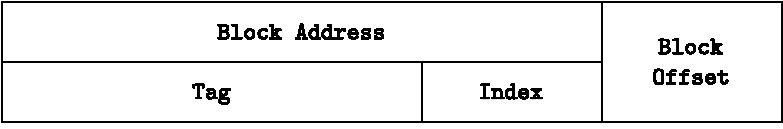
\includegraphics[width=.9\textwidth]{img/direct-mapped-cache-1.pdf}
    \caption{This figure shows the memory address composed of the block address (tag and index used to identify the block) and the block offset.}
    \label{fig: Memory Address - Direct Mapped Cache}
\end{figure}

\noindent
From Figure~\ref{fig: Direct Mapped Cache - Structure}, we can see the complete structure of the cache if we choose the direct mapped cache technique. 

\highspace
The rectangle on the top is the memory address (Figure~\ref{fig: Memory Address - Direct Mapped Cache}). First, we check the \emph{Tag} value; if it's equal to the value in the cache, we check the \emph{Valid bit} (V) to see if the position contains valid data: if the value is 1, we have a cache hit; otherwise, the data is invalid. The \emph{Tag} contains the value that univocally identifies the memory address corresponding to the stored data. To take the \emph{data word}, we use the \emph{block offset} as the \emph{selector} in the \href{https://en.wikipedia.org/wiki/Multiplexer}{multiplexer} to choose which data block to take. The index field indicates the cache row to check.

\newpage

\begin{figure}[!htp]
    \centering
    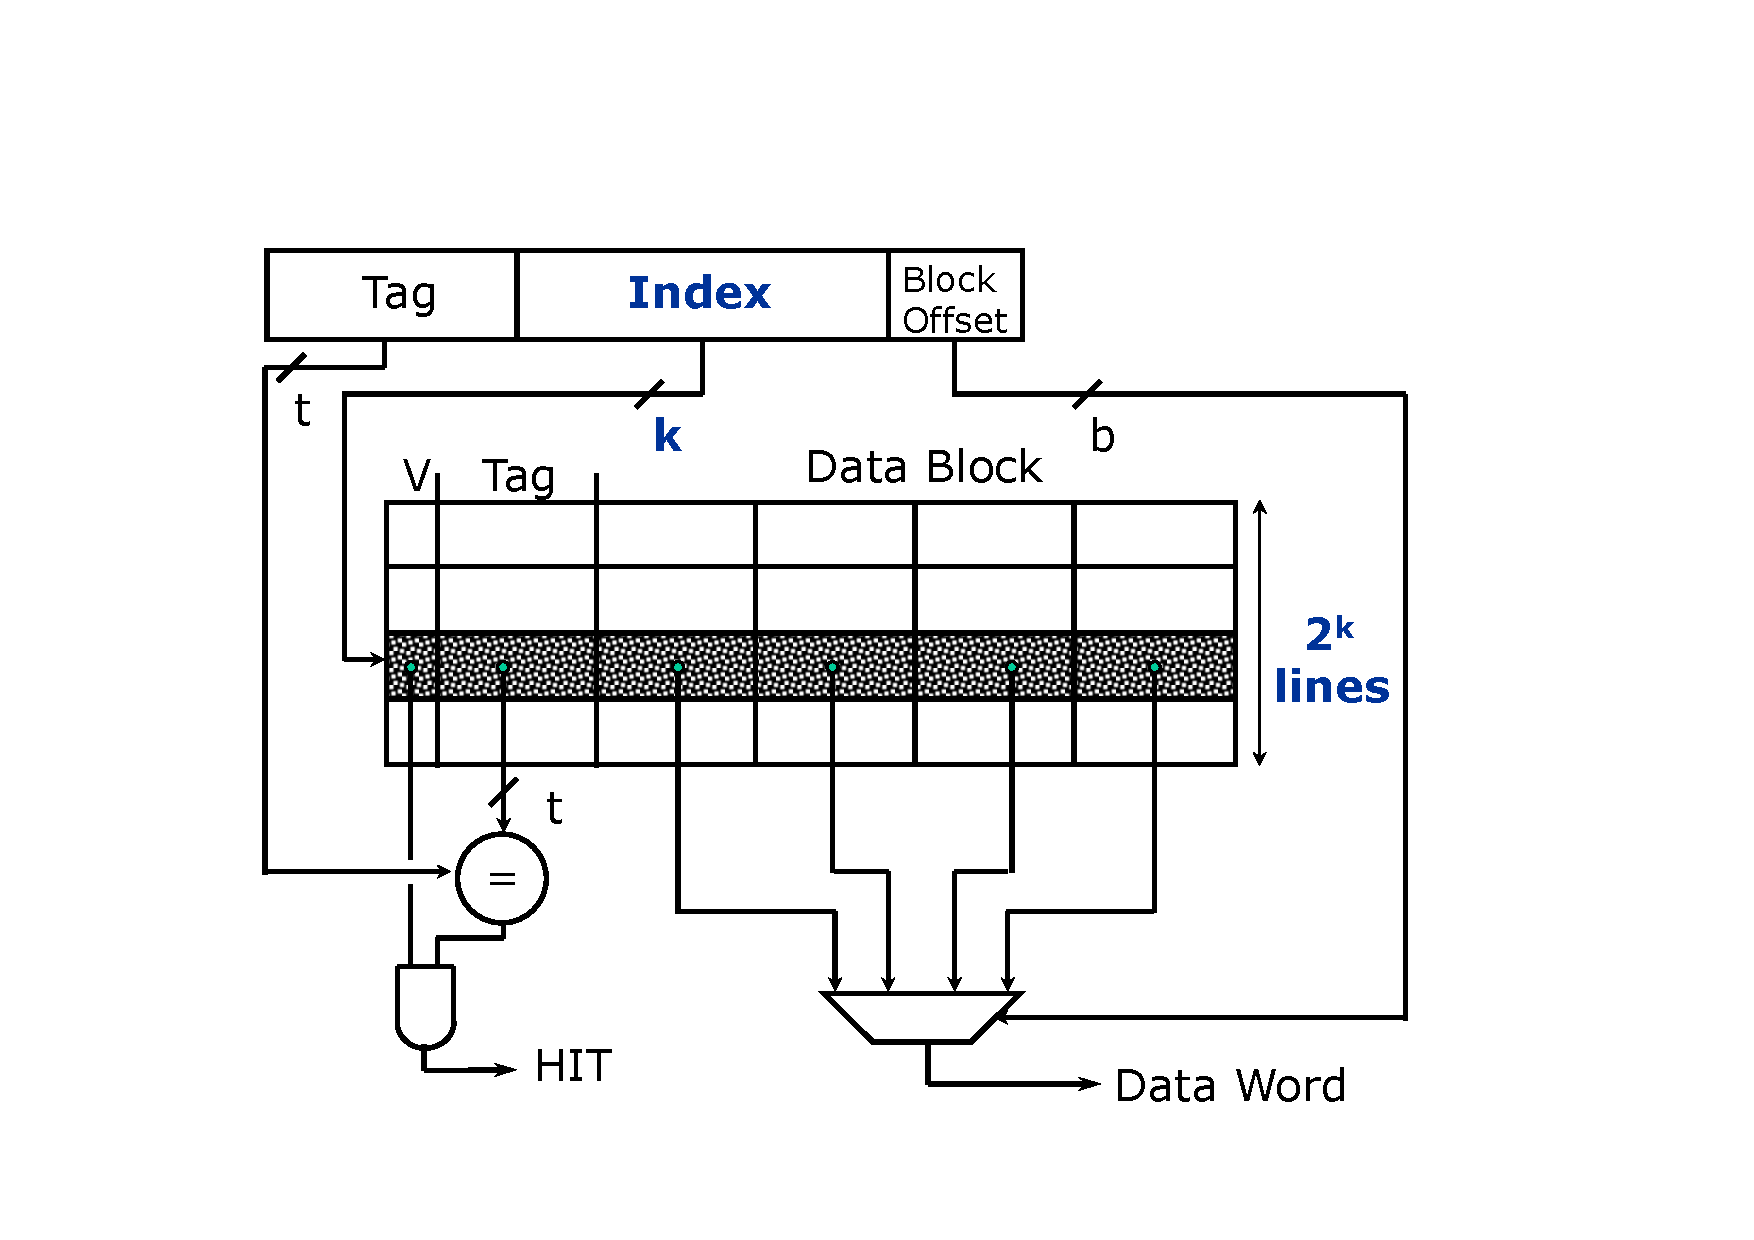
\includegraphics[width=.7\textwidth]{img/direct-mapped-cache-2.pdf}
    \caption{The cache structure of the \emph{Direct Mapped Cache} technique.}
    \label{fig: Direct Mapped Cache - Structure}
\end{figure}

\noindent
For \example{example}, we assume a block-frame address composed of 32 bits. Our cache structure is direct mapped, and the number of cache blocks is 8. A possible exercise could be \textbf{determining where block 12 can be placed in the 8-block cache}.

\highspace
To solve this problem, we can use the formula no \ref{eq: direct mapped cache} on page \pageref{eq: direct mapped cache}: 
\begin{equation*}
    \left(\texttt{Block Address}\right)_{\texttt{cache}} = 12 \mod 8 = 5
\end{equation*}
The result is $5$, so the answer is: with the direct mapped technique, \textbf{the block number is 4} (because the first index of the cache blocks is zero and not 1).

\begin{figure}[!htp]
    \centering
    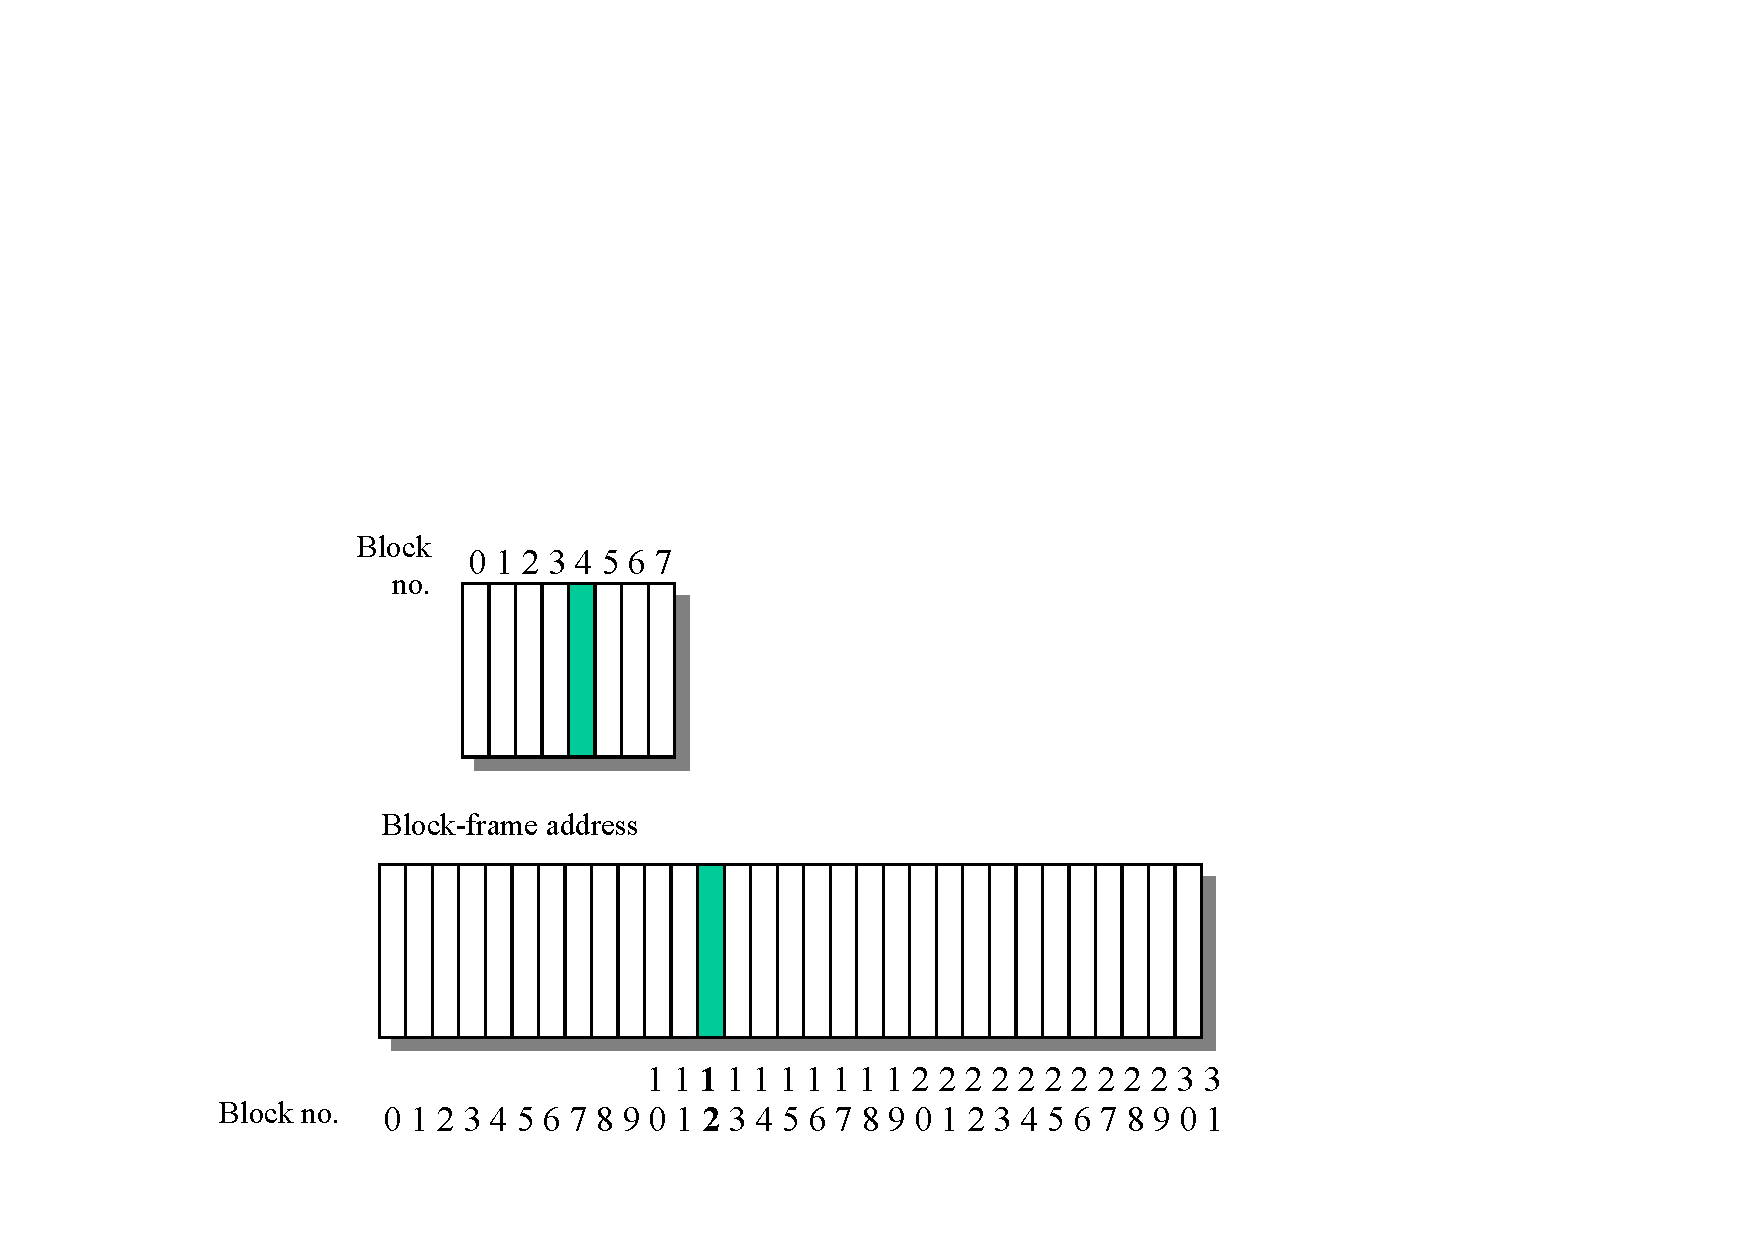
\includegraphics[width=.8\textwidth]{img/direct-mapped-cache-3.pdf}
\end{figure}

\newpage

\label{Fully Associative Cache}
\hypertarget{Fully Associative Cache}{\subsubsection*{\textcolor{Red2}{Fully Associative Cache}}}

In a \definition{Fully Associative Cache}, the \textbf{memory block can be placed in any position of the cache}. So, all the \textbf{cache blocks must be checked during the search of the block}.

\highspace
Note the \textbf{index does not exist} in the memory address; there are the Tag bits only:
\begin{equation}\label{eq: Fully Associative Cache}
    \texttt{Number of blocks} = \dfrac{\texttt{Cache Size}}{\texttt{Block Size}}
\end{equation}
The Memory Address comprises the Block Address (Tag) and the Block Offset.

\begin{figure}[!htp]
    \centering
    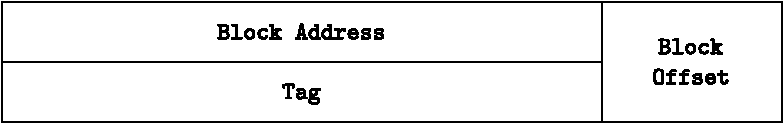
\includegraphics[width=.9\textwidth]{img/fully-associative-cache-1.pdf}
    \caption{The Memory Address comprises the Block Address (Tag) and the Block Offset.}
\end{figure}

\noindent
The structure of the cache using this technique is as follows:

\begin{figure}[!htp]
    \centering
    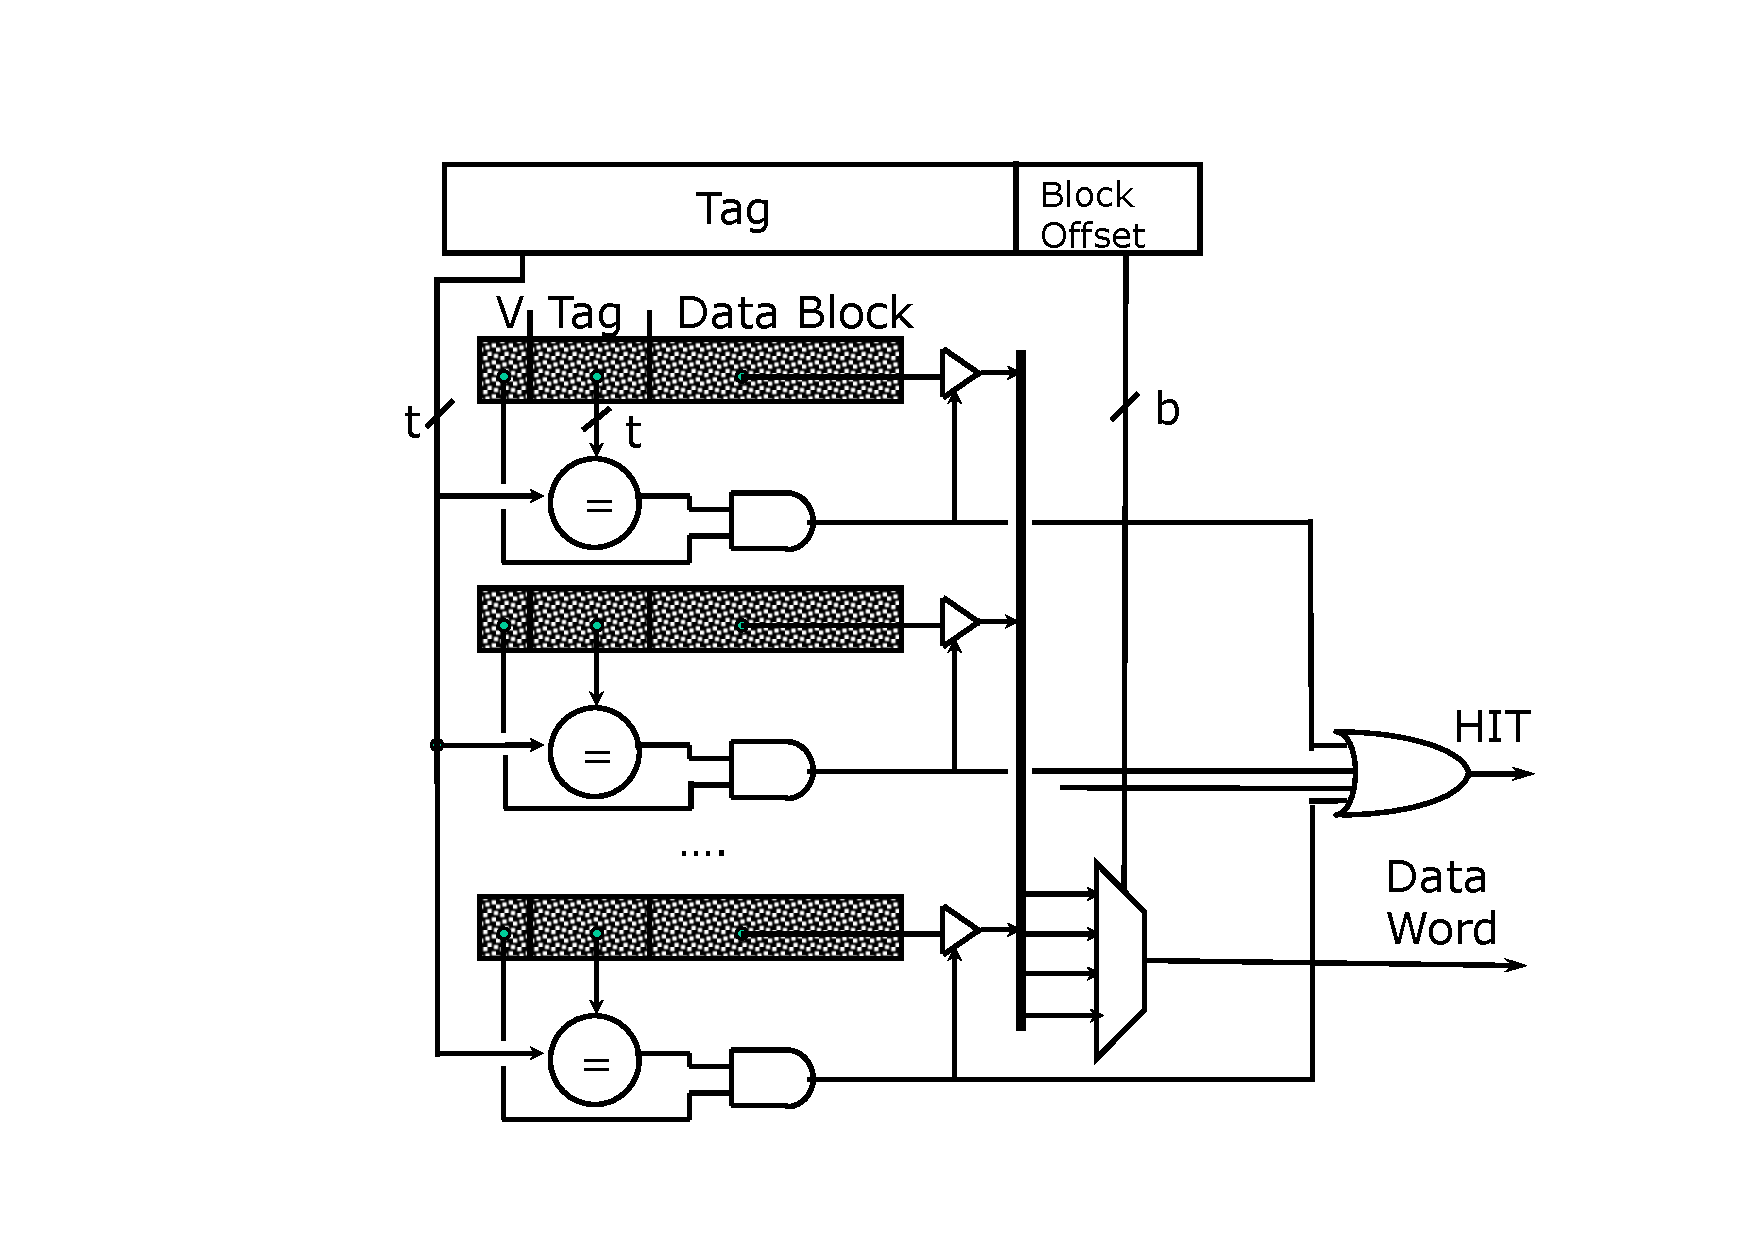
\includegraphics[width=.7\textwidth]{img/fully-associative-cache-2.pdf}
    \caption{The cache structure of the \emph{Fully Associative Cache} technique.}
    \label{fig: cache structure of the Fully Associative Cache}
\end{figure}

\noindent
As shown in Figure~\ref{fig: cache structure of the Fully Associative Cache}, the cache structure is more accessible because there are no \emph{Index} fields. We check only the \emph{Tag} field from the memory address. Finally, the \emph{Block Offset} chooses the \emph{Data Block} from the cache. We have a cache hit if the \emph{Tag} is equal to the \emph{Tag} of the cache and the value in and with the valid bit is true.

\newpage

\noindent
For \example{example}, we assume a block-frame address composed of 32 bits. Our cache structure is fully associative, and the number of cache blocks is 8. A possible exercise could be \textbf{determining where block 12 can be placed in the 8-block cache}.

\highspace
Unlike before, the position can be anywhere.

\begin{figure}[!htp]
    \centering
    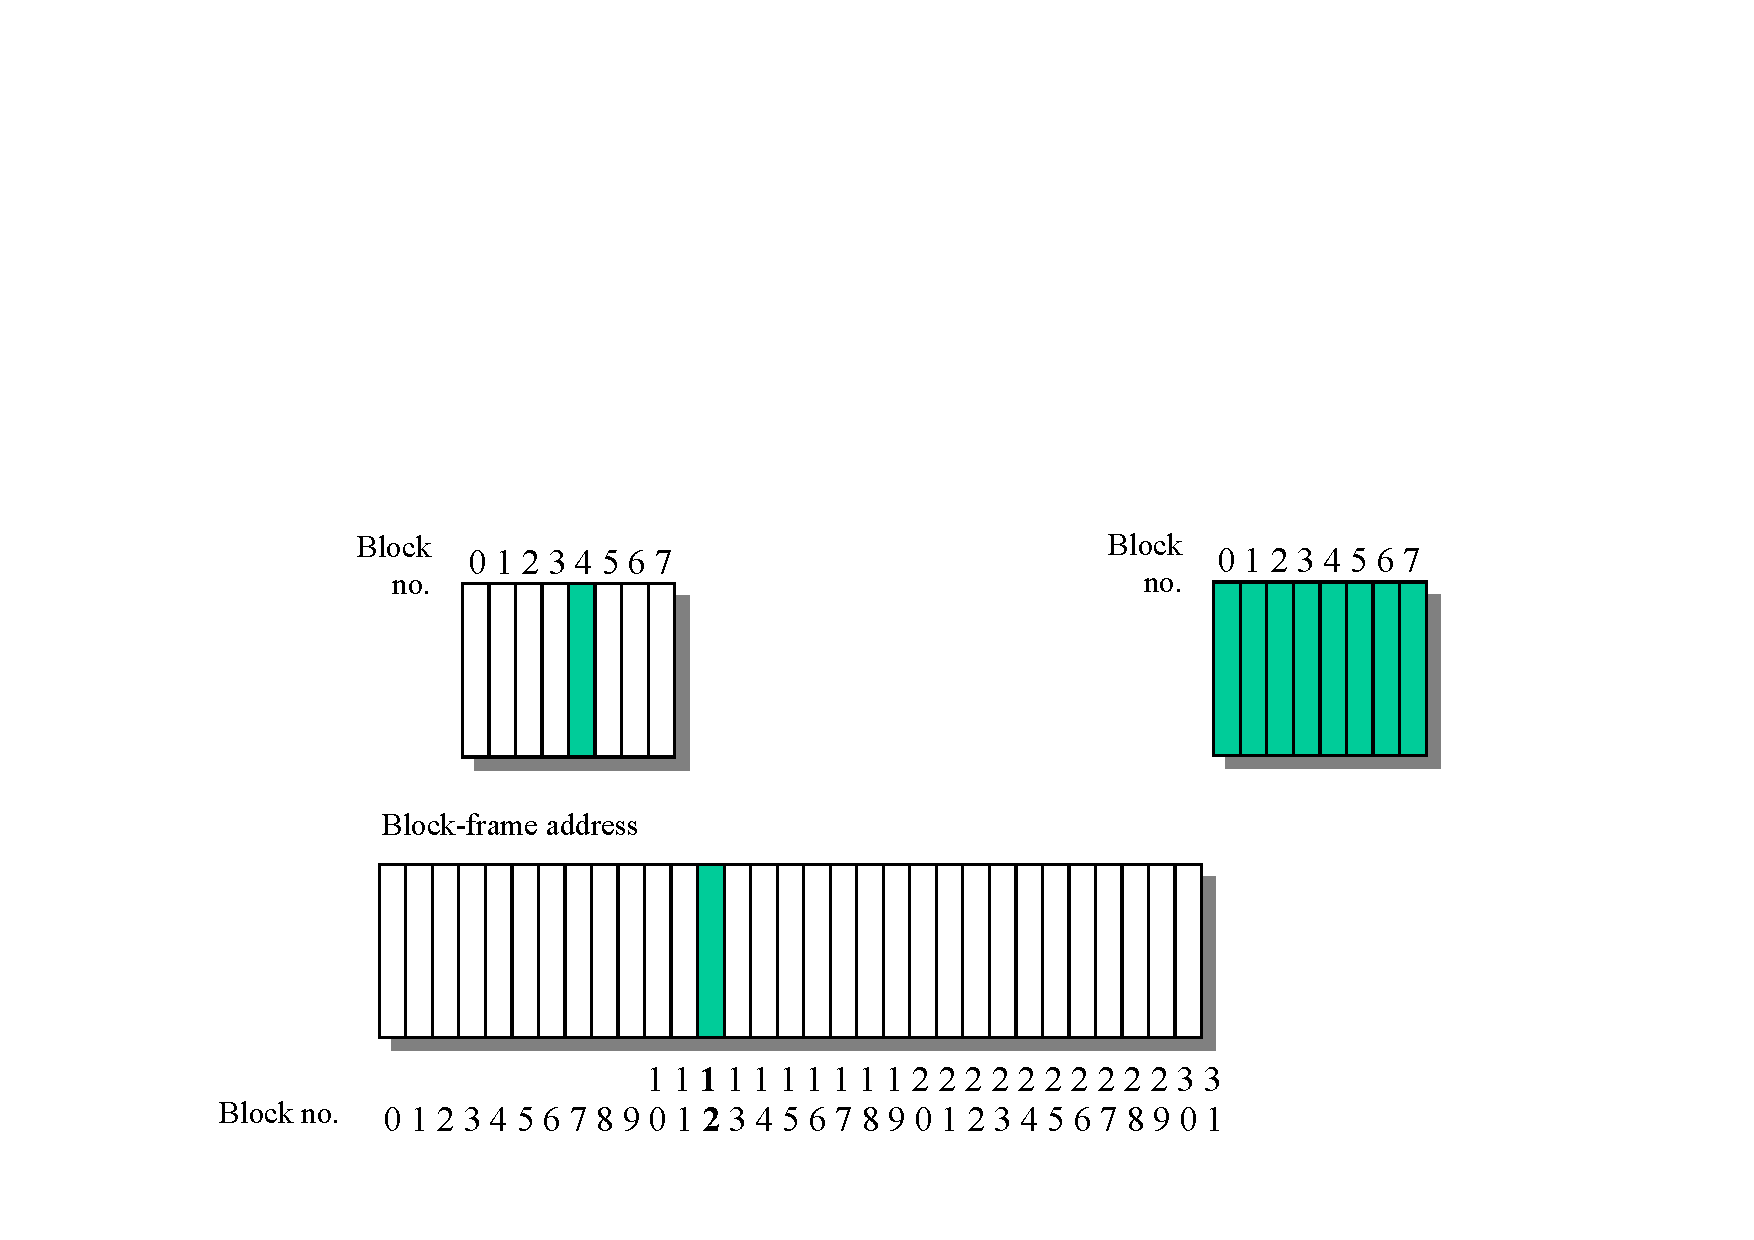
\includegraphics[width=.8\textwidth]{img/fully-associative-cache-3.pdf}
    \caption*{Direct Mapped on the left and Fully Associative on the right.}
\end{figure}

\newpage

\label{n-way Set Associative Cache}
\hypertarget{n-way Set Associative Cache}{\subsubsection*{\textcolor{Red2}{\emph{n}-way Set Associative Cache}}}

In a \definition{\emph{n}-way Set Associative Cache}, the \textbf{cache is composed of sets}. Each set is composed of \emph{n} blocks:
\begin{equation}
    \begin{array}{rcl}
        \texttt{Number of blocks} &=& \dfrac{\texttt{Cache Size}}{\texttt{Block Size}} \\ [1.5em]
        \texttt{Number of sets} &=& \dfrac{\texttt{Cache Size}}{\left(\texttt{Block Size} \times n\right)}
    \end{array}
\end{equation}
The memory block can be placed in any block of the set, so the \emph{search must be done on all the blocks}.

\highspace
\textbf{Each memory block corresponds to a single set of the cache}, and the \textbf{block can be placed in whatever block of the \emph{n} blocks of the set}:
\begin{equation}\label{eq: set cache}
    \left(\texttt{Set}\right)_{\texttt{cache}} = \left(\texttt{Block address}\right)_{\texttt{mem}} \texttt{mod} \left(\texttt{\# sets in cache}\right)
\end{equation}

\begin{figure}[!htp]
    \centering
    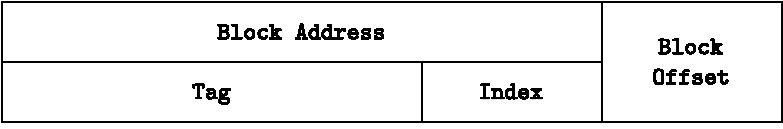
\includegraphics[width=.8\textwidth]{img/direct-mapped-cache-1.pdf}
    \caption{The memory address comprises the block address (Tag and index used to identify the set) and the block offset.}
\end{figure}

\begin{figure}[!htp]
    \centering
    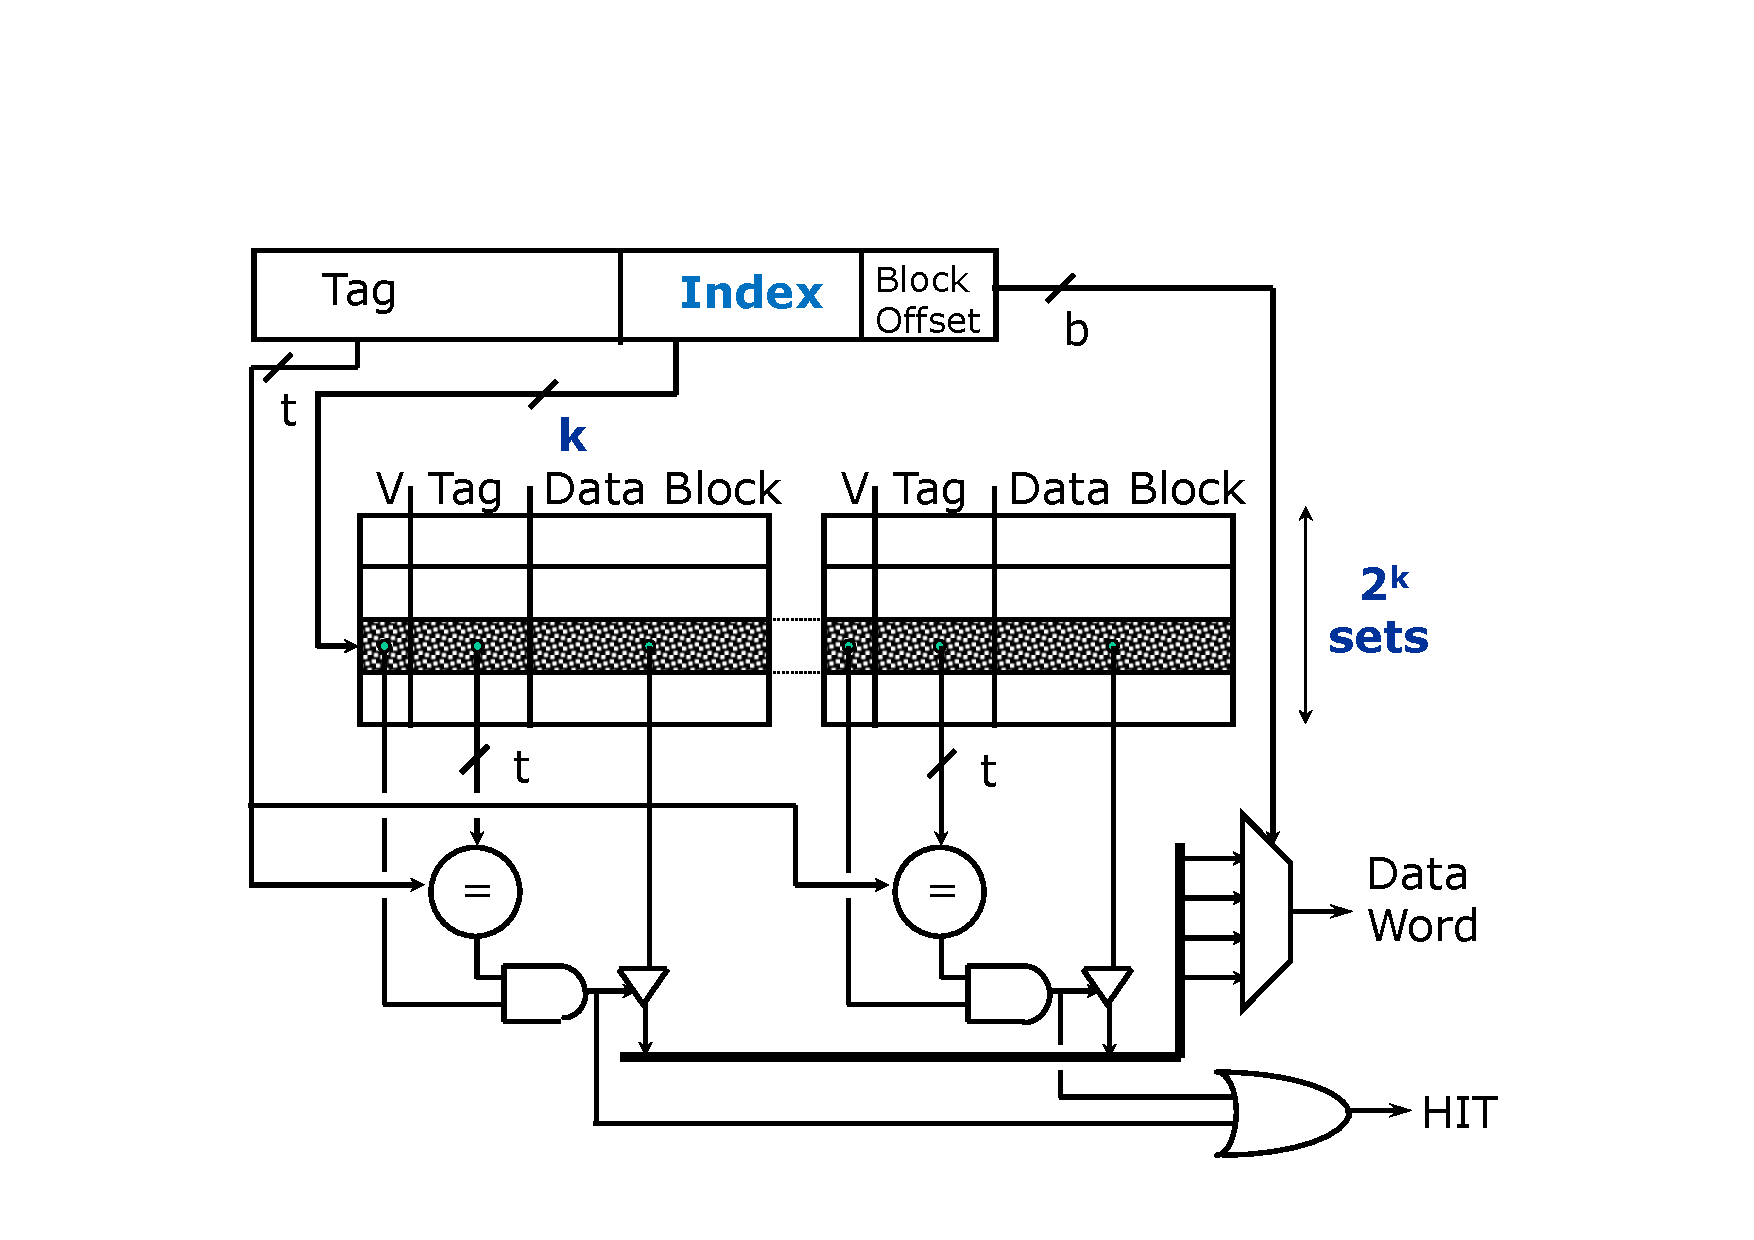
\includegraphics[width=.7\textwidth]{img/n-way-set-associative-cache-1.pdf}
    \caption{This structure is a \textbf{2-way Set Associative Cache}.}
\end{figure}

\newpage

\noindent
Taking the \example{examples} of previous pages, with the 2-way Set Associative, the answer is anywhere in set $0$. The reason for this is that using the formula~\ref{eq: set cache}:
\begin{equation*}
    \left(\texttt{Set}\right)_{\texttt{cache}} = 12 \mod 4 = 0
\end{equation*}

\begin{figure}[!htp]
    \centering
    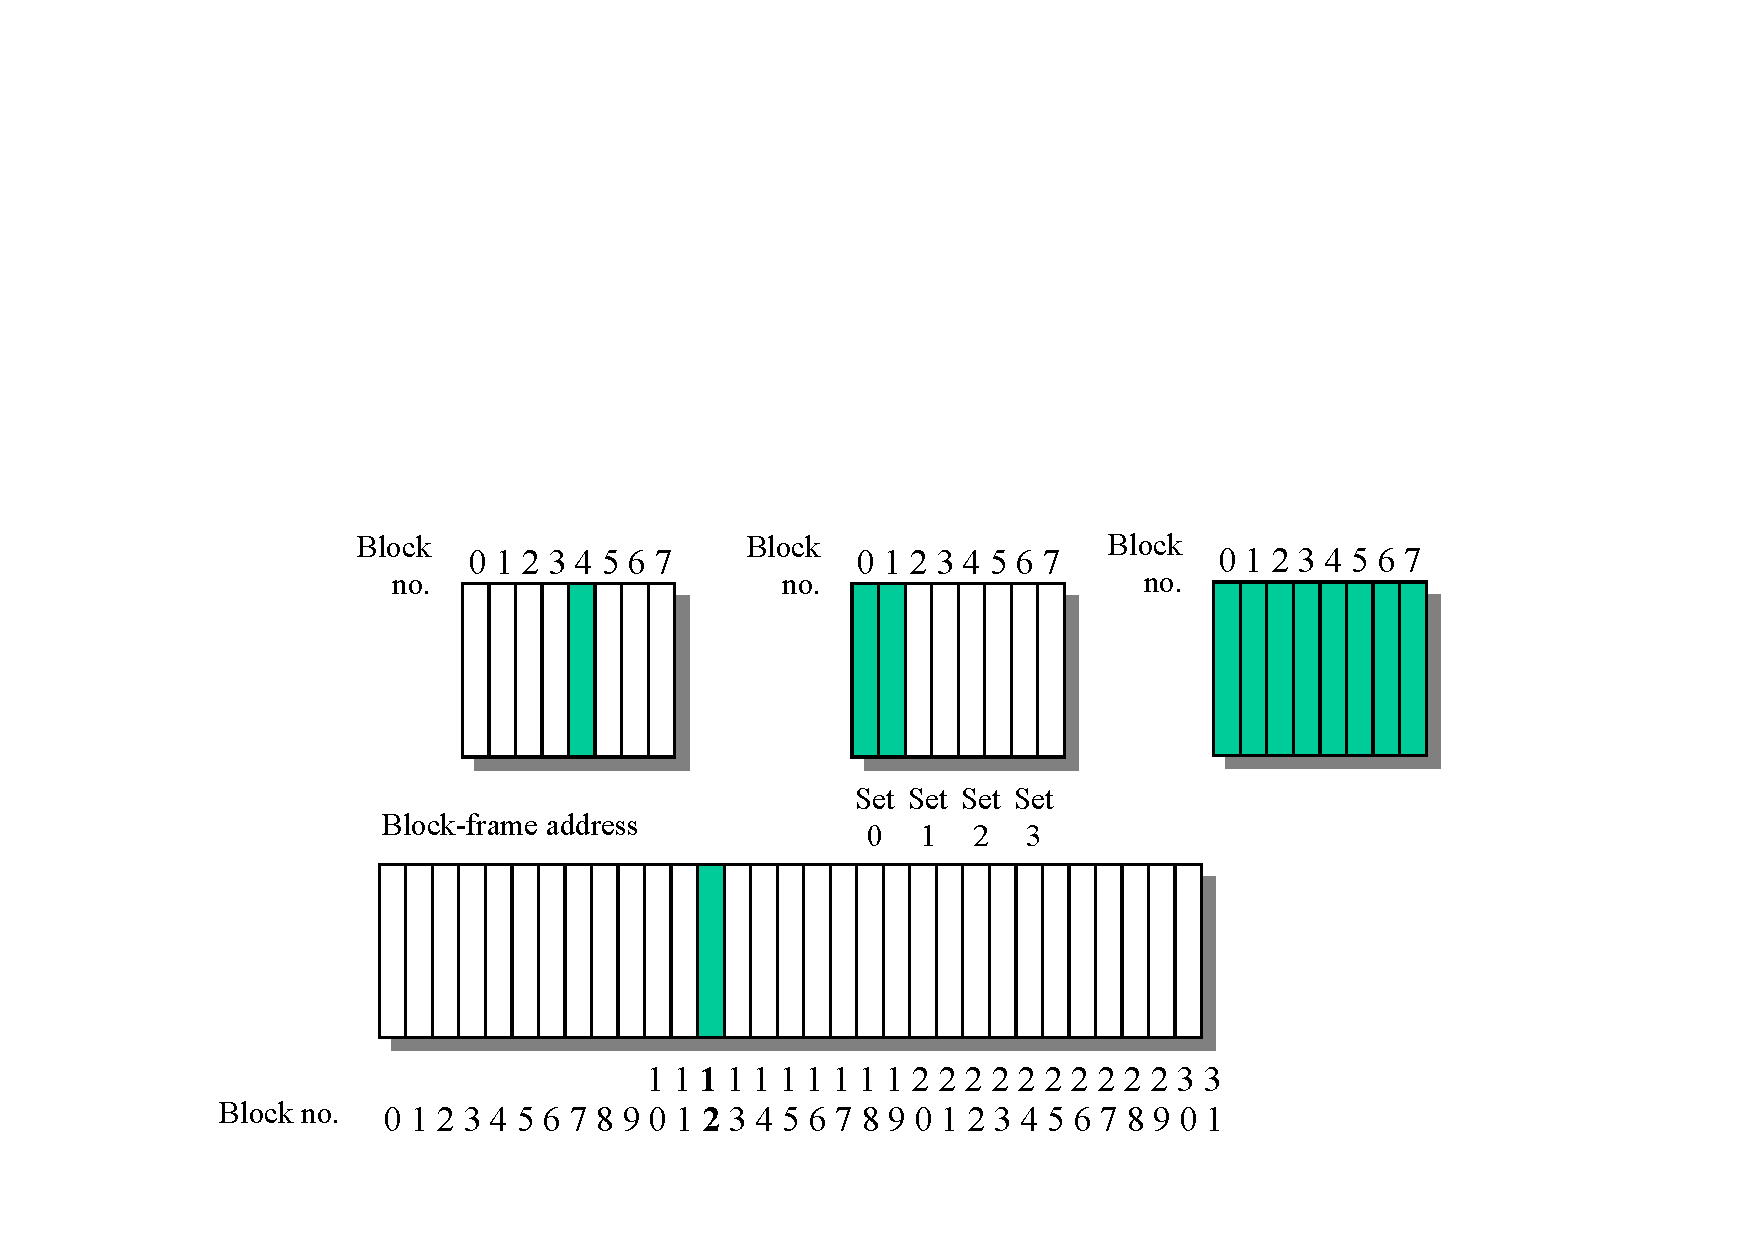
\includegraphics[width=\textwidth]{img/n-way-set-associative-cache-2.pdf}
    \caption*{Direct Mapped on the left, 2-way Set Associative on the center and Fully Associative on the right.}
\end{figure}

\newpage

\begin{center}
    \large
    \label{Block identification}
    \hypertarget{Block identification}{\textcolor{Red2}{\textbf{Block identification}}}
\end{center}

\noindent
The main question is: \emph{how is a block found if it is in the upper level?} The problem with identifying a block is that we must compare Tag bits. The comparison depends on the structure of the cache:
\begin{itemize}
    \item With \textbf{Direct Mapping} (page \pageref{Direct Mapped Cache}), we need to:
    \begin{itemize}
        \item Identify block positions by index (with the formula~\ref{eq: direct mapped cache});

        \item Compare block tags;
        
        \item Verify the valid bit.
    \end{itemize}

    \item With the \textbf{Set Associative Mapping} (page \pageref{n-way Set Associative Cache}), we need to:
    \begin{itemize}
        \item Identify the set by index (with the formula~\ref{eq: set cache});

        \item Compare tags of the set;

        \item Verify the Valid bit.
    \end{itemize}

    \item With the \textbf{Fully Associative Mapping} (page \pageref{Fully Associative Cache}), we must:
    \begin{itemize}
        \item Compare tags in \emph{every} block;
        
        \item Verify the Valid bit.
    \end{itemize}
\end{itemize}
Comparing the Tag bits, we do not need to check index or block offset bits.

\hfill

\longline

\hfill

\begin{center}
    \large
    \label{Block replacement}
    \hypertarget{Block replacement}{\textcolor{Red2}{\textbf{Block replacement}}}
\end{center}

\noindent
The main question is: \emph{which block should be replaced on a miss?} In case of a miss (definition on page~\pageref{definition: Cache Miss}), the replacement strategy depends on the structure of the cache:
\begin{itemize}
    \item In a \textbf{Fully Associative Cache} (page \pageref{Fully Associative Cache}), we need to decide which block to replace: any block is a potential candidate for the replacement.

    \item In a \textbf{Set Associative Cache} (page \pageref{n-way Set Associative Cache}), we must select among the blocks in the given set.
    
    \item In a \textbf{Direct Mapped Cache} (page \pageref{Direct Mapped Cache}), only one candidate must be replaced (\underline{no need} for any block replacement \underline{strategy}).
\end{itemize}
So in the \textbf{Fully Associative Cache} and \textbf{Set Associative Cache}, the \textbf{main strategies used to choose the block to be replaced} are:
\begin{itemize}
    \item \href{https://en.wikipedia.org/wiki/Cache_replacement_policies#Random_replacement_(RR)}{Random} (or \textbf{pseudo-random})
    
    \item \href{https://en.wikipedia.org/wiki/Cache_replacement_policies#Least_recently_used_(LRU)}{LRU (Least Recently Used)}

    \item \href{https://en.wikipedia.org/wiki/Cache_replacement_policies#First_in_first_out_(FIFO)}{FIFO (First In First Out, or oldest block replaced)}
\end{itemize}

\newpage

\begin{center}
    \large
    \label{Write strategy}
    \hypertarget{Write strategy}{\textcolor{Red2}{\textbf{Write strategy}}}
\end{center}

\noindent
The main question is: \emph{what happens on a write?} It depends on the written policy adopted in the cache. We remember that there are two possible options:
\begin{itemize}
    \item \definition{Write-Through}: \textbf{data is simultaneously updated} (written) \textbf{to cache and memory}. This process is more straightforward and more reliable. This is used when there are no frequent writes to the cache.
    
    \textcolor{Green3}{\faIcon{check} \textbf{The main advantages}}
    \begin{enumerate}
        \item It is \textbf{simpler to implement} but to be effective, it \emph{requires a write buffer} to not wait for the memory hierarchy (to avoid write stalls).

        \item The \textbf{read misses are cheaper} because they do not require any write to the memory hierarchy.

        \item \textbf{Memory is always up to date}. 
    \end{enumerate}


    \item \definition{Write-Back}: the \textbf{data is updated only in the cache and then added to the memory later}. The modified cache block is written to the memory only when it is replaced due to a cache miss. So, how can we understand if a block is clean or dirty? We need to add a \definition{Dirty Bit}. \textbf{Each Block in the cache requires a bit to indicate if the data present in the cache was modified} (\emph{Dirty}) \textbf{or not modified} (\emph{Clean}). If it is clean, writing it into the memory is unnecessary. It is designed to reduce write operation to a memory.

    \textcolor{Green3}{\faIcon{check} \textbf{The main advantages}}
    \begin{enumerate}
        \item The \textbf{processor can write the Block at the frequency the cache}, not the main memory, can accept.

        \item \textbf{Multiple writes to the same Block require only a single write to the main memory}.
    \end{enumerate}
\end{itemize}

\begin{flushleft}
    \textcolor{Red2}{\faIcon{question-circle} \textbf{What is a Write Buffer?}}
\end{flushleft}

\noindent
A \definition{Write Buffer} is a \textbf{FIFO buffer that does not wait for main memory access} (the typical number of entries is 4 to 8). So, the processor writes data to the cache and the write buffer; the memory controller writes the contents of the buffer to memory.

\begin{figure}[!htp]
    \centering
    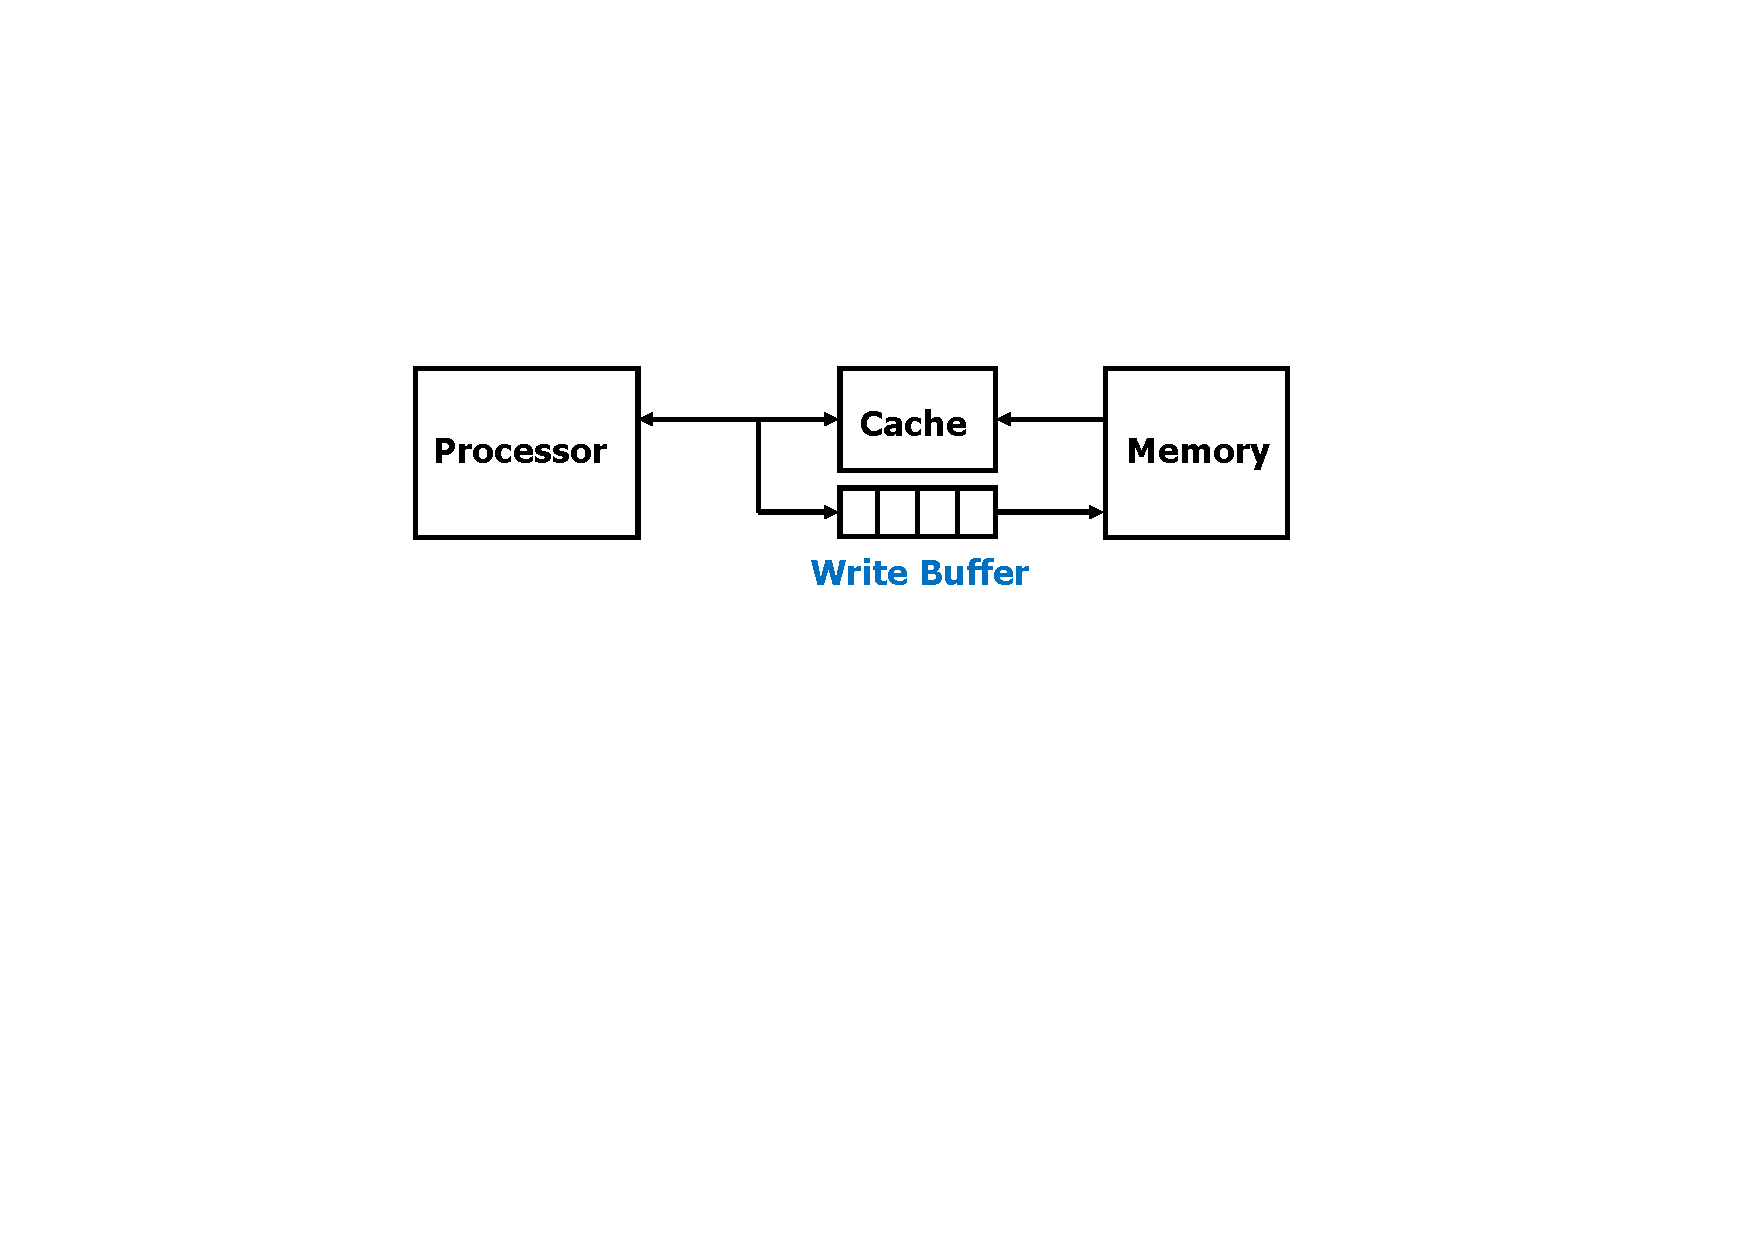
\includegraphics[width=.8\textwidth]{img/write-buffer-1.pdf}
    \caption{The cache structure with a Write Buffer.}
\end{figure}

\noindent
The \textbf{main problem with this idea is saturation}. However, as we have cited before, the write buffer is usually combined with the Write-Through policy.

\newpage

\begin{flushleft}
    \textcolor{Red2}{\faIcon{question-circle} \textbf{Ok, the cache can adopt one of the two write policies, but what happens on a Write Miss?}}
\end{flushleft}

\noindent
If write occurs to a location that is not present in the Cache (Write Miss), we use two options: \definition{Write Allocate} (or \emph{fetch on write}) and \definition{No Write Allocate} (\emph{Write-Around}). 

\highspace
In the first one, the \textbf{data is loaded from the memory into the cache and then updated}. Write Allocate works with both Write Back and Write-Through. However, it is \textbf{generally used with Write Back} because bringing data from the memory to the cache is unnecessary and then updating it in both the cache and main memory.

\highspace
In the \textbf{No Write Allocate} option, the \textbf{data is directly written/updated to the main memory without disturbing the cache}. It is better to use this when the data is not immediately used again. Generally, the \textbf{Write-Through cache uses the No Write Allocate} option (hoping the next writes to the Block will be done again in memory).

\newpage

\begin{flushleft}
    \textcolor{Green3}{\faIcon{clipboard-list} \textbf{Summary}}
\end{flushleft}

\begin{table}[!htp]
    \centering
    \begin{tabular}{@{} l p{20em} @{}}
        \toprule
        \textbf{Event} & \textbf{Summary} \\
        \midrule
        \textbf{Read Hit}   & Read data in cache. \\ [.5em]
        \textbf{Read Miss}  & Events that manifest themselves:
        \begin{enumerate}
            \item CPU stalls;
            \item Data request to memory;
            \item Copy in cache (write in cache);
            \item Repeat of cache read operation.
        \end{enumerate} \\
        \cmidrule{1-2}
        \textbf{Write Hit}  & It depends on the policy chosen:
        \begin{itemize}
            \item \emph{Write-Through}: write data both in cache and in memory.
            \item \emph{Write-Back}: write data to cache only, and copy memory only when replaced due to a cache miss.
        \end{itemize} \\ [.5em]
        \textbf{Write Miss} & There will certainly be CPU stalls. It also depends on the option we choose:
        \begin{itemize}
            \item \emph{Write Allocate}:
            \begin{enumerate}
                \item Data request to memory;
                \item Copy in cache (write in cache);
                \item Repeat of cache write operation.
            \end{enumerate}
            \item \emph{No Write Allocate}:
            \begin{enumerate}
                \item Simply send write data to main memory.
            \end{enumerate}
        \end{itemize} \\
        \bottomrule
    \end{tabular}
    \caption{Summary: Hit and Miss \& Read and Write.}
\end{table}